Having established the reduction to orientations,
and the symmetry-breaking assumption of canonicity,
we now turn to the construction of a CNF formula $\phi_n$
whose unsatisfiability would imply
that every set of $n$ points
contains a $6$-hole.\footnote{
  Satisfiability of $\phi_n$ would \emph{not} necessarily imply
  the existence of a point set without a $6$-hole.
  First, the mapping from sets of points to assignments of triple orientations is not surjective.
  Second, even if it were, $\phi_n$ is tailored to looking for an unsatisfiability proof,
  using implication rather than bi-implication in some of the variable-defining clauses.
}
The formula is detailed in~\Cref{fig:full-encoding}.

\begin{figure}
  \label{fig:full-encoding}
% \begin{framed}
  \begin{spreadlines}{16pt}
\begin{gather}
\hfsetfillcolor{green!10}
\hfsetbordercolor{green!60!black}
\tikzmarkin{b}(12.0,-0.9)(-0.5,0.5)
  \cvar_{i; a,b, c} \rightarrow \left(\left(\orvar_{a,b,c} \leftrightarrow \orvar_{a, i, c}  \right) \land \left(\orvar_{a,b,c} \leftrightarrow \ov{\orvar_{a, i, b}}  \right)\right) \text{ for all } 2 \leq a < i < b < c \leq n\label{eq:insideClauses1}\\
  \cvar_{i; a,b, c} \rightarrow \left(\left(\orvar_{a,b,c} \leftrightarrow \orvar_{a, i, c}  \right) \land \left(\orvar_{a,b,c} \leftrightarrow \ov{\orvar_{b, i, c}}  \right)\right) \text{ for all } 2 \leq a < b < i < c \leq n\label{eq:insideClauses2}\\
  \tikzmarkend{b}\Big(\bigwedge_{\substack{a < i < c\\ i \neq b}} \ov{\cvar_{i; a,b,c}}\Big) \rightarrow \hvar_{a, b, c} \quad \text{ for all } 2 \leq a < b < c \leq n\label{eq:holeDefClauses1}\\
%
\tikzmarkin{a}(12.0,-0.3)(-0.5,0.5)
  \orvar_{a, b, c} \land \orvar_{a, c, d} \rightarrow \orvar_{a, b, d} \quad \text{ for all } 2 \leq a < b < c < d \leq n\label{eq:signotopeClauses11}\\
  \tikzmarkend{a}\ov{\orvar_{a, b, c}} \land \ov{\orvar_{a, c, d}} \rightarrow \ov{\orvar_{a, b, d}} \quad \text{ for all } 2 \leq a < b < c < d \leq n \label{eq:signotopeClauses12}\\
%
\hfsetfillcolor{blue!10}
\hfsetbordercolor{blue!60!black}
\tikzmarkin{c}(12.0,-0.4)(-0.5,0.6)
  % \orvar_{1, b, c} \quad \text{ for all } 2 \leq b < c \leq n \label{eq:revLexClauses}\\
  \tikzmarkend{c}\left(\orvar_{\lceil \frac{n}{2} \rceil -1, \lceil \frac{n}{2} \rceil,\lceil \frac{n}{2} \rceil+1}, \ldots, \orvar_{2,3,4} \right) \succeq_{\text{lex}} \left(\orvar_{\lfloor \frac{n}{2}\rfloor +1,  \lfloor \frac{n}{2}\rfloor +2, \lfloor \frac{n}{2}\rfloor +3}, \ldots, \orvar_{n-2, n-1, n} \right)\label{eq:revLexClauses}\\
%
\hfsetfillcolor{orange!10}
\hfsetbordercolor{orange!60!black}
\tikzmarkin{d}(12.0,-0.3)(-0.5,0.5)
  \ov{\orvar_{a,b,c}} \land \ov{\orvar_{b,c,d}} \rightarrow \uvar_{a, c, d} \quad \text{ for all } 2 \leq a < b < c < d \leq n\label{eq:capDef}\\
  \orvar_{a, b, c} \land \orvar_{b, c, d} \rightarrow \vvar_{a, c, d} \quad \text{ for all } 2 \leq a < b < c < d \leq n \label{eq:cupDef}\\
  \uvar_{a,b,c} \land \ov{\orvar_{b,c,d}} \land \hvar_{a,b,d} \rightarrow \ufvar_{a, c, d} \quad \text{ for all } 2 \leq a < b < c < d \leq n,\; a+1<b\label{eq:capFDef}\\
  \uvar_{a, c, d} \rightarrow \ov{\orvar_{a,c,d}} \quad \text{ for all } 2 \leq a < c < d \leq n,\ a+1<c\label{eq:capDef2}\\
  \tikzmarkend{d}\vvar_{a, c, d} \rightarrow \orvar_{a,c,d} \quad \text{ for all } 2 \leq a < c < d \leq n,\; a+1<c\label{eq:cupDef2}\\
%
\hfsetfillcolor{red!10}
\hfsetbordercolor{red!60!black}
\tikzmarkin{e}(12.0,-0.5)(-0.5,0.5)
  \neg(\ufvar_{a,d,e} \land \orvar_{a, p, e}) \quad \text { for all } 2 \leq a < d < e \leq n, \; a < p < e, \; a+2 < d\label{eq:no6Hole1Below}\\
  \neg(\ufvar_{a,d,e} \land \ov{\orvar_{d, e, f}}) \quad \text { for all } 2 \leq a < d < e < f\leq n, \; a+2 < d\label{eq:no6Hole4Above}\\
  \neg(\uvar_{a,c,d} \land \vvar_{a, c', d} \land \hvar_{a,c,c'}) \quad \text{ for all } 2 \leq a < c < c' < d \leq n, \; a+1 < c\label{eq:no6Hole2Below1}\\
  \neg(\uvar_{a,c,d} \land \vvar_{a, c', d} \land \hvar_{a,c',c}) \quad \text{ for all } 2 \leq a < c' < c < d \leq n, \; a+1 < c'\label{eq:no6Hole2Below2}\\
  \tikzmarkend{e}\neg(\vvar_{a,c,d} \land \orvar_{c, d, e} \land \hvar_{a,c,e}) \quad \text{ for all } 2 \leq a < c < d < e \leq n, \; a+1 < c\label{eq:no6Hole3Below}
  \end{gather}
\end{spreadlines}
% \end{framed}
\caption{Encoding based on that of Heule and Scheucher for the Empty Hexagon Number~\cite{emptyHexagonNumber}. Each line determines a set of clauses. Unsatisfiability of the formula below for $n=30$ implies $h(6) \leq 30$, as detailed throughout the paper.}
\end{figure}


\subparagraph*{Variables.}
Let $S = (p_1, \ldots, p_n)$ be the list of points in canonical position.
We explain the variables of $\phi_n$
by specifying their values in the propositional assignment $\tau_S$
that is our intended model of $\phi_n$
corresponding to $S$. We then have:
\begin{itemize}
  \item
    For every $2 \leq a < b < c \leq n$, $\orvar_{a,b,c}$ is true
    iff $\sigma(p_a,p_b,p_c) = +1$.\footnote{
    Since the point set is in general position,
    we have $\neg \orvar_{a,b,c} \iff \sigma(p_a, p_b, p_c) = -1$.}

    The first optimization observes that orientations are antisymmetric:
    if $(p,q,r)$ is counterclockwise then $(q,p,r)$ is clockwise, etc.
    Thus one only needs $\orvar_{a,b,c}$ for ordered triples $(a,b,c)$,
    reducing the number of orientation variables by a factor of $3! = 6$
    relative to using all triples. The second optimization uses the \textbf{CCW-order} property of canonical positions:
    since all $\orvar_{1,a,b}$ are true, we may as well omit them from the encoding.

  \item
    Next, for every $a < b < c$ with $a < i < b$ or $b < i < c$,
    the variable $\cvar_{i;a,b,c}$ is true
    iff \lstinline|σPtInTriangle S[i] S[a] S[b] S[c]| holds.
    By \lstinline|σPtInTriangle_iff|, this is true exactly
    iff $p_i$ is inside the triangle $p_ap_bp_c$.

    The reason for assuming $(a,b,c)$ to be ordered is again symmetry:
    $p_ap_bp_c$ is the same triangle as $p_ap_cp_b$, etc.
    Furthermore thanks to the \textbf{$x$-order} property of canonical positions,
    if $p_i$ is in the triangle
    then $x(p_a) < x(p_i) < x(p_c)$.
    This implies that $a < i < c$,
    leaving one case distinction permuting $(i,b)$.

  \item
    For every $a < b < c$,
    $\hvar_{a,b,c}$ is true
    iff \lstinline|σIsEmptyTriangleFor S[a] S[b] S[c] S| holds.
    By a geometro-combinatorial connection analogous to ones above,
    this is true iff $p_ap_bp_c$ is a $3$-hole.

  \item
    Finally, one defines \emph{$4$-cap}, \emph{$5$-cap}, and \emph{$4$-cup} variables.
    For $a+1 < c < d$, $\uvar_{a,c,d}$ is true
    iff there is $b$ with $a < b < c$ with $\sigma(p_a,p_b,p_c) = \sigma(p_b,p_c,p_d) = -1$.
    $\vvar_{a,c,d}$ is analogous, except in that the two orientations are required to be counterclockwise.
    These are the $4$-caps and $4$-cups, respectively.
    The $5$-cap variables $\ufvar_{a,d,e}$
    are defined for $a+2 < d < e$.
    We set $\ufvar_{a,d,e}$ to true
    iff there exists $c$ with $a+1<c<d$
    such that $\uvar_{a,c,d}$, $\orvar_{c,d,e}$, and $\hvar_{a,c,e}$ are all true.

    Intuitively, $4$-caps and $4$-cups are clockwise and counterclockwise arcs of length $4$,
    respectively,
    whereas $5$-caps are clockwise arcs of length $5$ containing a $3$-hole.
    All three are depicted in [FIG].
\end{itemize}

\subparagraph*{Satisfaction.}
We now have to justify that the clauses of $\phi_n$
are satisfied by the intended interpretation $\tau_S$
for a $6$-hole-free point set $S$.
The variable-defining clauses~\labelcref{eq:insideClauses1,eq:insideClauses2,eq:holeDefClauses1,eq:capDef,eq:cupDef,eq:capFDef,eq:capDef2,eq:cupDef2}
follow essentially by definition combined with boolean reasoning.
The orientation properties~\labelcref{eq:signotopeClauses11,eq:signotopeClauses12}
have been established in the family of theorems \lstinline|σ_propᵢ|.
The lexicographic ordering clauses~\labelcref{eq:revLexClauses}
follow from the \textbf{Lex order} property of canonical positions.
Thus we are left with clauses~\labelcref{eq:no6Hole1Below,eq:no6Hole4Above,eq:no6Hole2Below1,eq:no6Hole2Below2,eq:no6Hole3Below}
which forbid the presence of certain $6$-holes.\footnote{
They are intended to forbid \emph{all} $6$-holes,
but we do not prove completeness.}
Justifying these is by far the most complicated
part of the proof.
We illustrate it for clause~\labelcref{eq:no6Hole1Below}.
It is easier to state the contrapositive:
if $\tau_S(\ufvar_{a,d,e}) = \tau_S(\orvar_{a,b,e}) = 1$,
then $S$ contains a $6$-hole.
To show this, we need to introduce \lstinline{Arc}s, \lstinline|σCCWPoints|,
and prove two key lemmas.

\begin{lstlisting}
inductive Arc (w : CanonicalPoints) (o : Orientation) :
    List (Fin w.length) → Prop where
  | one : a < b → Arc w o [a, b]
  | cons : a < b →
    σ w[a] w[b] w[c] = o → Arc w o (b::c::l) → Arc w o (a::b::c::l)

def σCCWPoints : List Point → Prop
  | [] => True
  | a :: l => l.Pairwise (σ a · · = .ccw) ∧ σCCWPoints l
\end{lstlisting}

\textbf{Triangulations.} Given any convex point set $S$
and a line $\overleftrightarrow{ab}$ between vertices of $S$,
the convex hull of $S$ is contained in the convex hull
of points on each side of $\overleftrightarrow{ab}$. That is:
\begin{lstlisting}
theorem split_convexHull (cvx : ConvexPoints S) :
  ∀ {a b}, a ∈ S → b ∈ S →
    convexHull ℝ S ⊆
    convexHull ℝ {x ∈ S | σ a b x ≠ ccw} ∪
    convexHull ℝ {x ∈ S | σ a b x ≠ cw}
\end{lstlisting}
By using this lemma repeatedly, we can slice up a convex $k$-gon into smaller pieces in any way we like until we get to triangles, thereby showing that convex polygons can be triangulated. We will use this in particular to show that a hexagon can be covered by only 4 triangles, instead of the ${6\choose 3}$ triangles required by the previous lemma.
\begin{figure}
    \centering
    \begin{subfigure}{0.45\textwidth}
        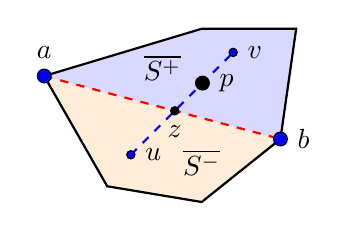
\begin{tikzpicture}
        \coordinate (a) at (0, 0.4);
        \coordinate (b) at (3, -0.4);
        \coordinate (v1) at (3.2, 1);
        \coordinate (v2) at (2, 1);
        \coordinate (u1) at (0.8, -1);
        \coordinate (u2) at (2, -1.2);
        \coordinate (u) at (1.1, -0.6);
        \coordinate (v) at (2.4, 0.7);
        \coordinate (p) at (2.01,0.31);
        \coordinate (z) at (1.65789, -0.0421053);

        \fill[blue, opacity=0.15] (b) -- (v1) -- (v2) -- (a) -- cycle;
        \fill[orange, opacity=0.15] (a) -- (u1) -- (u2) -- (b) -- cycle;

        \draw[thick] (a) -- (u1) -- (u2) -- (b) -- (v1) -- (v2) -- (a);
        \draw[dashed, thick, red] (a) -- (b);
        \draw[dashed, thick, blue] (u) -- (v);

        \node[draw, circle, black, fill=blue, inner sep=0pt, minimum size=5pt, label=above:$a$] (pA) at (a) {};
        \node[draw, circle, black, fill=blue, inner sep=0pt, minimum size=5pt, label=right:$b$] (pB) at (b) {};
        \node[draw, circle, black, fill=blue, inner sep=0pt, minimum size=3pt, label=right:$u$] (pU) at (u) {};
        \node[draw, circle, black, fill=blue, inner sep=0pt, minimum size=3pt, label=right:$v$] (pV) at (v) {};

        \node[draw, circle, black, fill=black, inner sep=0pt, minimum size=5pt, label=right:$p$] (pP) at (p) {};
        \node[draw, circle, black, fill=black, inner sep=0pt, minimum size=3pt, label=below:$z$] (pZ) at (z) {};

        \node[] at (1.5, 0.5) {$\overline{S^+}$};
        \node[] at (2, -0.7) {$\overline{S^-}$};

        \end{tikzpicture}
        \caption{}\label{fig:triangulation2-a}
    \end{subfigure}
    \begin{subfigure}{0.45\textwidth}
        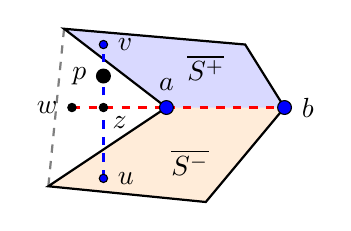
\begin{tikzpicture}
            \coordinate (a) at (1.5, 0);
            \coordinate (b) at (3, 0);
            \coordinate (v1) at (2.5, 0.8);
            \coordinate (v2) at (0.2, 1);
            \coordinate (u1) at (0, -1);
            \coordinate (u2) at (2, -1.2);
            \coordinate (u) at (0.7, -0.9);
            \coordinate (v) at (0.7, 0.8);
            \coordinate (p) at (0.7, 0.4);
            \coordinate (z) at (0.7, 0);
            \coordinate (w) at (0.3, 0);

            \fill[blue, opacity=0.15] (b) -- (v1) -- (v2) -- (a) -- cycle;
            \fill[orange, opacity=0.15] (a) -- (u1) -- (u2) -- (b) -- cycle;

            \draw[thick] (a) -- (u1) -- (u2) -- (b) -- (v1) -- (v2) -- (a);
            \draw[dashed, thick, red] (a) -- (b);
            \draw[dashed, thick, blue] (u) -- (v);
            \draw[dashed, thick, red] (w) -- (a);
            \draw[dashed, thick, opacity=0.5] (v2) -- (u1);

            \node[draw, circle, black, fill=blue, inner sep=0pt, minimum size=5pt, label=above:$a$] (pA) at (a) {};
            \node[draw, circle, black, fill=blue, inner sep=0pt, minimum size=5pt, label=right:$b$] (pB) at (b) {};
            \node[draw, circle, black, fill=blue, inner sep=0pt, minimum size=3pt, label=right:$u$] (pU) at (u) {};
            \node[draw, circle, black, fill=blue, inner sep=0pt, minimum size=3pt, label=right:$v$] (pV) at (v) {};

            \node[draw, circle, black, fill=black, inner sep=0pt, minimum size=5pt, label=left:$p$] (pP) at (p) {};
            \node[draw, circle, black, fill=black, inner sep=0pt, minimum size=3pt, label={[shift={(-0.05,0.05)}]-45:$z$}] (pZ) at (z) {};
            \node[draw, circle, black, fill=black, inner sep=0pt, minimum size=3pt, label=left:$w$] (pW) at (w) {};

            \node[] at (2, 0.5) {$\overline{S^+}$};
            \node[] at (1.8, -0.7) {$\overline{S^-}$};

        \end{tikzpicture}
        \caption{}\label{fig:triangulation2-b}
    \end{subfigure}
    \caption{Illustration of the proof for \lstinline|split_convexHull|. (a) Given point $p$, we obtain points $u$ and $v$ inside the two halves and $z$ as the point of intersection with the line $\overline{ab}$. (b) In this (contradictory) situation, the point $z$ has ended up outside the segment $\overline{ab}$, because $S$ is not actually convex. In this case we construct $w$ such that $z$ is on the $\overline{wa}$ segment, and observe that $w,z,a,b$ are collinear.}\label{fig:triangulation2}
\end{figure}

\begin{proof}
    Let $S^+=\{x\in S\mid \sigma(a,b,x)\ge 0\}$ and $S^-=\{x\in S\mid \sigma(a,b,x)\le 0\}$ be the two sets in the theorem, and let $p\in \overline{S}$, where $\overline{S}$ denotes the convex hull of $S$. Assume WLOG that $\sigma(a,b,p)\ge 0$. (We would like to show that $p\in \overline{S^+}$.) Now $p$ is a convex combination of elements of $S^+$ and elements of $S^-$, so there exist points $u\in \overline{S^-}$ and $v\in \overline{S^+}$ such that $p$ lies on the $\overline{uv}$ line.

    Because $\{x\mid \det(a,b,x)\le 0\}\supseteq S^-$ is convex, it follows that $\det(a,b,u)\le 0$, and likewise $\det(a,b,v)\ge 0$, so they lie on opposite sides of the $\overleftrightarrow{ab}$ line and hence $\overline{uv}$ intersects $\overleftrightarrow{ab}$ at a point $z$. The key point is that $z$ must in fact be on the line segment $\overline{ab}$; assuming that this was the case, we could obtain $z$ as a convex combination of $a$ and $b$, and $p$ as a convex combination of $v$ and $z$, and since $v$ is in $\overline{S^+}$ and $a,b\in S^+\subseteq\overline{S^+}$ we can conclude $p\in \overline{S^+}$.

    To show that $z\in \overline{ab}$, suppose not, so that $a$ lies between $z$ and $b$ (see \Cref{fig:triangulation2-b}). (The case where $z$ is on the $b$ side is similar.) We can decompose $z$ as a convex combination of some $w\in \overline{S\setminus\{a\}}$ and $a$, which means that $w,z,a,b$ are collinear and appear in this order on the line. Therefore $a$ is a convex combination of $w$ and $b$, which means that $a\in \overline{S\setminus\{a\}}$ which violates convexity of $S$.
\end{proof}

\textbf{Joining arcs.} two arcs can be put together into a \lstinline|σCCWPoints|
% theorem Arc.join (H1 : Arc w .ccw (a::l₁++[b])) (H2 : Arc w .cw (a::l₂++[b])) :
%    σCCWPoints ((a::l₁++b::l₂.reverse).map (w[·])) := by

% theorem satisfies_no6Hole1Below {w : CanonicalPoints} (hw : ¬σHasEmptyKGonIf 6 holes w.toFinset)
%    {a d e f : Fin w.rlen} (ae : a < e) (ef : e < f) :
%    (no6Hole1Below a d f e).eval (w.toPropAssn holes) := by
%  simp [no6Hole1Below]; intro ⟨df, c, ⟨b, ab, bc, cd, abc, bcd⟩, cdf, acf⟩ aef
%  have := Arc.join (l₁ := [_]) (l₂ := [_,_,_])
%    (.cons' ae aef <| .one' ef)
%    (.cons' ab abc <| .cons' bc bcd <| .cons' cd cdf <| .one' df)
%  refine hw <| this.emptyHexagonIf w.gp (acf · |>.perm₂) (subset_map' w [a, e, f, d, c, b])

\begin{proof}[Proof of clause~\labelcref{eq:no6Hole1Below}]
any \lstinline|σCCWPoints| containing a $3$-hole must form a $6$-hole.
% TODO inline proof of
% theorem σCCWPoints.emptyHexagon
%    (H : σCCWPoints [a, b, c, d, e, f]) (gp : Point.ListInGenPos S)
%    (hole : σIsEmptyTriangleFor a c e S.toFinset) (sp : [a, b, c, d, e, f] ⊆ S) :
%    σHasEmptyKGon 6 S.toFinset := by
\end{proof}

\subparagraph*{QED.}
Having now shown that if $\phi_{30}$ were unsatisfiable,
our main result would follow,
we run a distributed computation to confirm the antecedent
and conclude the proof.
